\chapter{Módulo de Gestión de Empleados} \label{chp:gestion_empleados}

Este capítulo está dedicado a detallar el cuarto módulo principal del sistema, el cual se centra en la gestión de los empleados asociados a una empresa. En primer lugar, se explica la operativa y los permisos necesarios para llevar a cabo el registro de un nuevo trabajador, así como la posterior edición de su información. A continuación, se detalla de forma exhaustiva la estructura y categorización de los datos que conforman el formulario de alta de empleados, abarcando desde la identificación básica hasta los datos de formación, detalles de contrato y las constantes internas necesarias para las integraciones oficiales.

%7.1
\section{Operativa de Empleados: Alta y Edición}

La funcionalidad troncal de este módulo es la creación de nuevos registros de trabajadores para una entidad u organización específica, así como el mantenimiento seguro de dicha información a lo largo del tiempo.

%7.1.1
\subsection{Proceso de Registro y Permisos (revisar)}

Para poder crear un empleado, el usuario debe contar con permisos de ``rrhh'' (recursos humanos). Una vez que el usuario cuenta con este rol, está autorizado para acceder al registro de nuevos empleados a través de un formulario específico en el frontend. Este formulario recoge toda la información legal, de contacto, residencia y contractual del trabajador, que posteriormente se comunicará a la TGSS para formalizar el alta técnica.



\begin{figure}[H]
    \centering % Sustituye la ruta por el nombre de tu archivo de imagen
    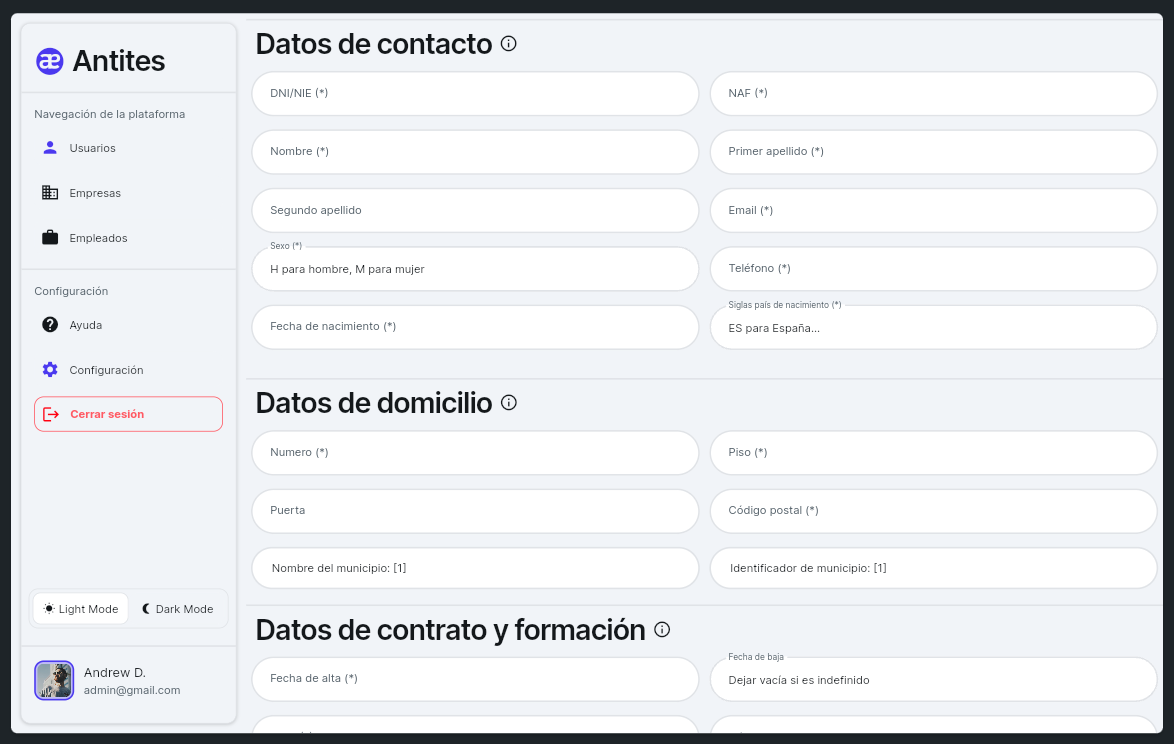
\includegraphics[width=0.8\textwidth]{imagenes/07_CrearEmpleado.png}
    \caption{Formulario de Alta de Empleado}
    \label{fig:crear_empleado}
\end{figure}

Tras completar el formulario y confirmar el registro, el sistema enviará al endpoint facilitado por la empresa la información del nuevo empleado, lo que a su vez desencadenará la comunicación automática con la TGSS para formalizar el alta técnica. Es importante destacar que el proceso de alta en la plataforma y el proceso de alta en la Seguridad Social son dos acciones distintas pero interconectadas, siendo esta última una consecuencia directa del registro en el sistema.

%7.1.2
\subsection{Edición de Datos y Trazabilidad}

Si se ha cometido un error en la introducción de datos o si es necesario actualizar la información de un empleado, el usuario con permisos de ``rrhh'' también tiene la capacidad de editar los registros existentes. La edición se realiza a través de una interfaz similar al formulario de alta, pero con los campos pre-cumplimentados con los datos actuales del empleado, lo que permite una actualización eficiente y sin errores.

Al igual que en el capítulo anterior, el menú de edición de empleados difiere del de creación en que aparece un botón en la zona superior derecha para eliminar al empleado, y en que, en vez de aparecer en la parte inferior de la página el botón de ``Añadir usuario'', aparece un botón de ``Guardar cambios'' para confirmar la actualización de los datos.
        

%7.2
\section{Datos del Formulario de Empleados}
En esta sección, se va a explicar en detalle qué datos se recogen en el formulario. Aunque ya se ha hablado de ello en los apartados anteiores, las imágenes adjuntadas en dichos apartados no muestran al completo el formulario, por lo que se ha considerado necesario dedicar un apartado específico para detallar cada uno de los campos que se recogen en el mismo.

Para formalizar el registro o la edición, el usuario debe rellenar un formulario que recoge toda la información legal, de contacto, residencia y contractual del empleado.

Estos datos se estructuran lógicamente en los siguientes apartados:

%7.2.1
\subsection{Datos de Identificación y Contacto}

Esta sección agrupa la información personal primaria del trabajador, así como los identificadores necesarios para los trámites legales y de afiliación a los organismos públicos.

%7.2.1.1
\subsubsection{Identificación Oficial y Afiliación} El sistema requiere especificar en primer lugar el \textbf{Tipo de Documento} de identificación (por ejemplo, DNI, NIE o Pasaporte). Esta selección define qué formato y valor se guardará en el campo contiguo, el \textbf{DNI/NIE}, el cual actúa como la clave principal de identificación fiscal y laboral del empleado. Adicionalmente, es obligatorio introducir el \textbf{NAF} (Número de Afiliación a la Seguridad Social), un identificador único del trabajador ante la Tesorería General de la Seguridad Social (TGSS), indispensable para tramitar y validar cualquier alta.

%7.2.1.2
\subsubsection{Filiación y Datos Personales} Se deben recoger los datos básicos de filiación: \textbf{Nombre, Apellido1 y Apellido2}, los cuales sirven como identificación formal en el contrato, en la propia comunicación del alta y en la posterior generación de nóminas. También se solicita el \textbf{Sexo} (género del trabajador), un dato necesario para cumplimentar el Modelo 145 del IRPF y para ciertos trámites estadísticos de la TGSS. Otro campo estrictamente obligatorio es la \textbf{Fecha de nacimiento}, fundamental para la verificación de la identidad y de la edad legal del trabajador ante la Seguridad Social. Por último, se debe indicar el \textbf{ID País}, que identifica el país de nacionalidad del empleado y es crucial para diferenciar entre trabajadores comunitarios y extracomunitarios.

%7.2.1.3
\subsubsection{Información de Contacto} El formulario incluye un campo para el \textbf{Teléfono}, que recoge el número de contacto directo del trabajador. Aunque este dato no es estrictamente obligatorio para formalizar el alta técnica en la TGSS, se utilizará en la plataforma para facilitar la comunicación interna y agilizar posibles trámites administrativos.

%7.2.2
\subsection{Datos de Domicilio}

Esta sección del formulario está destinada a registrar la residencia legal del empleado, estrictamente necesaria para la emisión de notificaciones y la correcta aplicación de la normativa.

%7.2.2.1
\subsubsection{Dirección Física y Geográfica} Para conformar la dirección de manera estandarizada, se solicita el \textbf{Tipo de vía pública} (por ejemplo, CL para calle, AV para avenida, PZ para plaza), un dato exigido por la Agencia Tributaria y la TGSS para el formato oficial del domicilio. A este campo le sigue la \textbf{Vía pública}, que recoge el nombre de la calle o avenida y forma parte del domicilio fiscal. Para detallar la ubicación exacta dentro del edificio, se deben rellenar los campos correspondientes al \textbf{Número de la calle, piso y puerta}. Finalmente, es imperativo introducir el \textbf{ID municipio}, el cual actúa como identificador del municipio del domicilio y es un requisito ineludible para las comunicaciones a Hacienda y al SEPE.

Para reforzar la confianza en que el usuario haya introducido correctamente este último dato, al lado del código postal de la dirección se muestra el nombre del municipio asociado al ID introducido, lo que permite una verificación visual inmediata y reduce la probabilidad de errores en la introducción de este dato crítico.

%7.2.3
\subsection{Datos de Contrato y Formación}

Este bloque asienta las bases de la relación laboral entre el trabajador y la organización empleadora.

%7.2.3.1
\subsubsection{Vinculación Corporativa y Académica} En primer lugar, se requiere el \textbf{ID de la Empresa} (código CCC), un campo esencial para la segregación de datos que vincula inequívocamente al empleado con su empresa. A continuación, se establece la \textbf{Fecha de alta}, que marca el inicio de la relación laboral y es la fecha exacta que se comunica a la TGSS; esta debe estar comprendida entre el día en el que se realiza el alta y 60 días posteriores. A nivel formativo, se solicita el \textbf{ID del nivel de estudios}, que indica el nivel máximo alcanzado por el trabajador, un dato que solicita de forma obligatoria el SEPE en la comunicación de contratos a través del sistema Contrat@.

%7.2.3.2
\subsubsection{Condiciones y Datos Bancarios} El formulario requiere seleccionar el \textbf{ID del convenio}, el identificador del Convenio Colectivo aplicable, el cual queda enlazado al campo “Código Convenio” de la entidad empresa y define las condiciones salariales mínimas del puesto. Para la futura gestión de la nómina, se recoge el \textbf{IBAN} (Código Internacional de Cuenta Bancaria), que indica la cuenta bancaria donde el trabajador recibirá sus ingresos y que debe ser custodiado con alta seguridad y cifrado. Por último, y para perfiles laborales concretos, se solicita el \textbf{Número de Tarjeta de Conductor} (tarjeta de tacógrafo), siendo esto imprescindible para el cumplimiento de la normativa en el sector del transporte.

%7.2.4
\subsection{Constantes (Uso Futuro y Lógica de Contrato)}

Además de los datos visibles y rellenados manualmente, el sistema contempla una serie de variables internas o constantes destinadas a automatizar lógicas futuras, generación de documentos y la integración transparente con los sistemas del Estado.

%7.2.4.1
\subsubsection{Parámetros Oficiales de Seguridad Social} Se establece el campo \textbf{Situación} (por defecto "01"), que determina la situación inicial en la Seguridad Social (Alta en Régimen General) y se comunica mediante el fichero TA.2/S. A su vez, se define el \textbf{Tipo de contrato} (por ejemplo, 100 para indefinido, 420 para temporal), un código oficial que categoriza la relación laboral y dictamina posibles bonificaciones o penalizaciones por parte de la TGSS. Este se complementa con el \textbf{Subtipo de contrato}, que detalla la modalidad específica requerida por el SEPE. Asimismo, se incluye el \textbf{Colectivo del trabajador}, que recoge códigos específicos de colectivos singulares (como personas con discapacidad) necesarios para la correcta aplicación de reducciones de cuotas en la TGSS.

%7.2.4.2
\subsubsection{Condiciones Laborales y Retributivas} La plataforma registra el \textbf{Porcentaje de jornada}, un coeficiente de parcialidad (por ejemplo, 100 para jornada completa, 50 para media jornada) que afecta de forma directa y proporcional a la cotización a la Seguridad Social. A esto se le suma el \textbf{Horario}, que aloja una descripción del horario de trabajo, siendo un dato contractual obligatorio para el correcto registro de jornada. En el apartado económico, el sistema gestiona el \textbf{Importe bruto}, es decir, el salario anual o mensual bruto del trabajador que servirá como base para el cálculo de la nómina y la base de cotización, junto con el \textbf{Tipo de importe}, que especifica la periodicidad del pago (anual, mensual o por hora).

%7.2.4.3
\subsubsection{Temporalidad, Antigüedad y Periodo de Prueba} Para los contratos de duración determinada, es obligatorio registrar la \textbf{Fecha de fin de contrato} para su comunicación al SEPE, así como el \textbf{Motivo de la temporalidad} (circunstancias de la producción, sustitución, etc.), que conforma la justificación legal ineludible exigida para el cumplimiento del Real Decreto-ley 32/2021. Finalmente, se establecen como datos contractuales clave la duración del \textbf{Periodo de prueba} aplicable al inicio de la actividad, y el campo \textbf{Antigüedad}, que actuará como variable de control interno para el futuro cálculo automatizado de trienios o complementos dentro del módulo de generación de nóminas.
